\documentclass[acmsmall,screen,nonacm]{acmart}

\usepackage{filecontents}
\usepackage{graphicx}
\usepackage{hyperref}
\usepackage{geometry}
\usepackage{array}
\usepackage{fancyhdr}
\usepackage[margin=1in]{geometry}
\usepackage{parskip}
\usepackage{setspace}
\usepackage{tabularx}
\usepackage{amssymb}
\usepackage{float}
\usepackage{tikz}
\usetikzlibrary{shapes.geometric, arrows.meta, positioning, fit, calc}
\usepackage{listings}

\setstretch{1.08}

\makeatletter
\makeatother

\pagestyle{fancy}
\fancyhf{} 

\begin{document}


\begin{center}
    {\Huge \textbf{Real-Time Wildfire Resilience Digital Twin}} \\
    \vspace{0.5em}
    {\Large \textbf{Group Name: N-Dimensional}} \\
    \vspace{2em}

    \hspace*{-1.5cm} 
    \begin{tabular}{ >{\centering\arraybackslash}p{3.8cm} >{\centering\arraybackslash}p{3.8cm} >{\centering\arraybackslash}p{3.8cm} >{\centering\arraybackslash}p{3.8cm} }
        
        \textbf{Prince Savsaviya}\textsuperscript{*} & \textbf{Viswanadh R. Challa}\textsuperscript{*} & \textbf{Anish Ashok Kale}\textsuperscript{*} & \textbf{Ali Rezayi Nejad}\textsuperscript{*} \\
        
        \small ID: 862548420 & \small ID: 862548873 & \small ID: 862547289 & \small ID: 862392323 \\
        
        \small UC Riverside & \small UC Riverside & \small UC Riverside & \small UC Riverside \\
        
        \small \href{mailto:psavs001@ucr.edu}{psavs001@ucr.edu} & 
        \small \href{mailto:vchal008@ucr.edu}{vchal008@ucr.edu} & 
        \small \href{mailto:akale014@ucr.edu}{akale014@ucr.edu} & 
        \small \href{mailto:areza018@ucr.edu}{areza018@ucr.edu} \\
        
    \end{tabular}
    
    \vspace{1em}
    {\footnotesize \textsuperscript{*}Department of Computer Science, University of California, Riverside}
    \vspace{2em}
\end{center}

\date{March 17, 2026}


\section*{Abstract}
This project builds a real-time wildfire digital twin designed to assess and visualize risk to critical infrastructure. The goal is to ingest high-volume continuous data streams—such as live fire occurrences and weather conditions—and perform rapid spatial intersections against a statewide database of 11.5 million building footprints. The key idea leverages a decoupled, distributed architecture utilizing Apache Kafka for event streaming, Apache Spark with Sedona for spatial processing, DuckDB for low-latency analytical querying, and Uber's H3 geospatial indexing for lightning-fast localized rendering. Our main result demonstrates that by replacing inefficient Python User-Defined Functions (UDFs) with Sedona native expressions and leveraging H3 partitions within GeoParquet, the system achieves an end-to-end P95 processing latency of under 30 seconds for bursts of 1,000 concurrent fire events, ensuring real-time interactivity.

\section{Introduction}
Wildfires represent an increasingly severe threat to life, property, and critical infrastructure. As the frequency and intensity of these events rise due to environmental shifts \cite{abatzoglou2016impact, doerr2016global}, emergency responders and planners require robust tools to instantly assess the risk posed by active fires to nearby facilities, such as hospitals, schools, and emergency stations. Traditional geographic information systems (GIS) are often bottlenecked by static data workflows and struggle to dynamically process high-velocity data streams in real time \cite{li2020realtime}.

To address this challenge, we developed a dynamic data-driven application system (DDDAS). The main contribution of this project is a scalable, end-to-end digital twin pipeline that continuously assimilates live weather and fire-event streams, calculates directional fire-spread risk zones, and rapidly identifies threatened infrastructure across a dataset of 11.5M buildings in California. We introduce a decoupled architecture that utilizes Kafka, Spark Structured Streaming, and DuckDB to separate high-throughput ingestion from dashboard analytical reads. 

Our initial implementation exhibited a P95 latency of over 215 seconds, precluding real-time functionality. Through rigorous optimization—specifically replacing Python UDFs with native Sedona spatial expressions and implementing H3 Hexagon-based partitioning—we successfully reduced the P95 latency to approximately 18.65 seconds for a load of 1,000 simultaneous fire events. This optimization enables interactive simulation workflows within a highly responsive Streamlit dashboard.

The remainder of this report is structured as follows: Section 2 categorizes related work and grounds our project within existing literature. Section 3 provides a high-level overview of our proposed digital twin architecture. Sections 4, 5, and 6 delve into the specific details of the ingestion, geospatial processing, and analytical layers. Section 7 presents our evaluation methodology and results. Finally, Section 8 highlights our conclusions and Section 9 details specific author contributions.

\section{Related Work}
Our system bridges several disciplines, drawing upon foundational research categorized below:

\textbf{Digital Twin and DDDAS Frameworks:} The concept of a digital twin, a tightly coupled virtual representation of a physical system, was originally established by Grieves \cite{grieves2014digitaltwin}. Darema further formalized the Dynamic Data-Driven Application Systems (DDDAS) paradigm, enabling simulations to dynamically incorporate online data \cite{darema2004dddas}. Our work directly translates these theories into a functional prototype for disaster response.

\textbf{Geospatial Streaming and Big Data:} Scalable real-time tracking requires robust stream processing. Zaharia et al. introduced Apache Spark as a unified engine for large-scale data processing \cite{zaharia2016spark}, while Kreps et al. detailed Kafka's distributed logging capabilities \cite{kreps2011kafka}. Our spatial operations are heavily reliant on GeoSpark/Sedona, introduced by Yu et al. \cite{yu2019geospark}, to execute clustered spatial joins effectively.

\textbf{Fire Spread and Risk Modeling:} Fire spread forecasting relies heavily on models like Rothermel's surface spread equations \cite{rothermel1972spread} and operational tools like FARSITE \cite{finney1998farsite}. While physics-based models (e.g., FIRETEC \cite{linn2002firetec}) exist, they require high computational costs. To maintain $<30s$ latency, our system utilizes a heuristic vector-based spread envelope (wind cones) driven by live weather variables.

This project relates to these categories by prioritizing low latency, combining robust open-source big-data tools (Kafka, Spark, DuckDB) into a lightweight, deployable pipeline tailored specifically for infrastructure risk assessment.

\section{System Architecture Overview}
The Wildfire-Twin architecture is designed to decouple real-time write-heavy event processing from read-heavy geospatial visualizations. The pipeline consists of four main components (see Figure \ref{fig:arch}):

\begin{figure}[h]
\centering
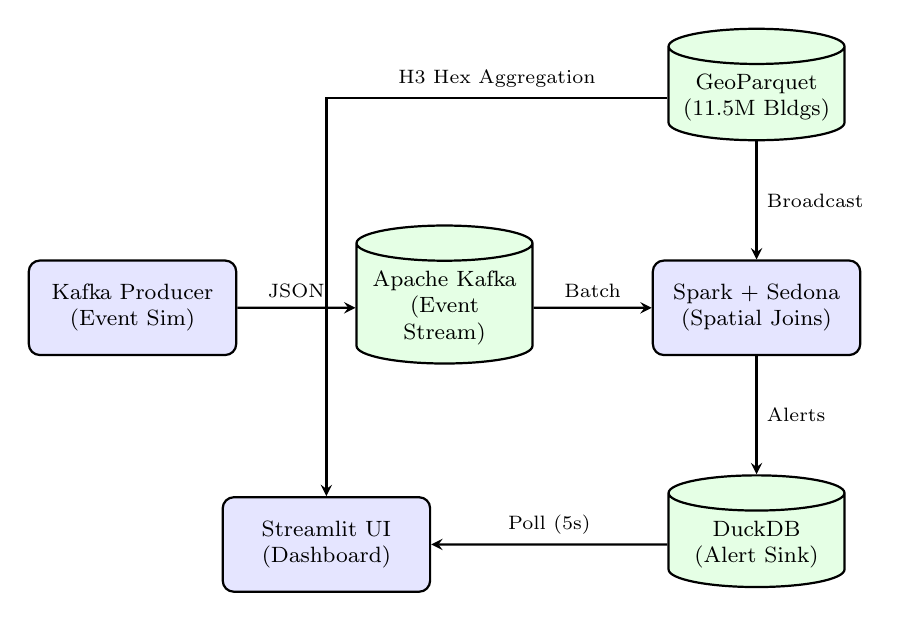
\begin{tikzpicture}[
  node distance=1cm and 1.5cm,
  box/.style={rectangle, draw=black, thick, fill=blue!10, text width=2.4cm, align=center, rounded corners, minimum height=1.2cm, font=\footnotesize},
  db/.style={cylinder, draw=black, thick, aspect=0.2, shape border rotate=90, fill=green!10, text width=2cm, align=center, minimum height=1.2cm, font=\footnotesize},
  arrow/.style={thick, ->, >=stealth, font=\scriptsize}
]

\node[box] (producer) {Kafka Producer\\(Event Sim)};
\node[db, right=of producer] (kafka) {Apache Kafka\\(Event Stream)};
\node[box, right=of kafka] (spark) {Spark + Sedona\\(Spatial Joins)};
\node[db, below=of spark, yshift=-0.5cm] (duckdb) {DuckDB\\(Alert Sink)};
\node[box, left=of duckdb, xshift=-1.5cm] (streamlit) {Streamlit UI\\(Dashboard)};
\node[db, above=of spark, yshift=0.5cm] (geoparquet) {GeoParquet\\(11.5M Bldgs)};

\draw[arrow] (producer) -- node[above] {JSON} (kafka);
\draw[arrow] (kafka) -- node[above] {Batch} (spark);
\draw[arrow] (geoparquet) -- node[right] {Broadcast} (spark);
\draw[arrow] (spark) -- node[right] {Alerts} (duckdb);
\draw[arrow] (duckdb) -- node[above] {Poll (5s)} (streamlit);
\draw[arrow] (geoparquet) -| node[above, near start] {H3 Hex Aggregation} (streamlit);

\end{tikzpicture}
\caption{System Architecture of the decoupled Wildfire Digital Twin.}
\label{fig:arch}
\end{figure}

\begin{enumerate}
    \item \textbf{Ingestion Layer:} A Python/Kafka producer script ingests live (e.g., NASA FIRMS) or simulated fire events, combined with real-time weather metadata, into a durable Kafka topic \cite{wang2015kafka, narkhede2017kafka}.
    \item \textbf{Geospatial Processing Engine:} An Apache Spark cluster running Apache Sedona \cite{yu2015geospark} ingests the Kafka stream using Structured Streaming \cite{armbrust2018structured}. It constructs directional wind-cone polygons based on weather data and performs distributed spatial joins against the partitioned state-wide building GeoParquet dataset.
    \item \textbf{Analytical Storage Sink:} Spark outputs matched "At-Risk" events back to Kafka. A lightweight Python consumer ingests these alerts and maintains a sliding window of state inside a DuckDB live store \cite{raasveldt2019duckdb}, taking advantage of columnar analytical performance \cite{abadi2008column}.
    \item \textbf{Interactive Dashboard:} A Streamlit application built with PyDeck and Folium provides the user interface for visual data analytics \cite{keim2008visual}. It reads from the DuckDB store and the H3-partitioned \cite{brodsky2018h3, sahr2003geodesic} GeoParquet file to render live alerts and infrastructure risk maps interactively.
\end{enumerate}

\section{Spatial Data Preparation and Indexing}
Processing 11.5M building footprints concurrently against a streaming spatial join requires meticulous data preparation.

\subsection{Semantic Enrichment}
The core dataset comprises 11.5 million Microsoft building footprints combined with 79,000 OpenStreetMap Points of Interest (POIs). Because standard spatial joins between these two layers at runtime severely impact performance, we implemented \textit{offline semantic categorization}. 

During an offline preprocessing step, string manipulation heuristics are applied directly to the `building\_type` field (e.g., matching "Hospital" or "Clinic" to denote "Medical", and "School" to denote "Education"). This eliminates the need for a secondary runtime spatial join to identify critical facilities, drastically reducing the Directed Acyclic Graph (DAG) complexity within Spark.

\subsection{H3 Geospatial Partitioning}
To further expedite loading and map rendering, the enriched GeoDataFrame is partitioned fully using Uber's H3 indexing system. The dataset is organized into physical directory partitions at H3 Resolution 7.

This partitioned approach provides a dual benefit:
\begin{itemize}
    \item \textbf{Partition Pruning:} Spark can prune directories during the spatial join, avoiding full table scans.
    \item \textbf{Dashboard Rendering:} At statewide zoom levels, parsing 11.5M GeoJSON features causes browser crashes. Instead, the Streamlit dashboard seamlessly performs a `value\_counts()` aggregation over the `h3\_res7` partition keys and utilizes PyDeck's native \texttt{H3HexagonLayer} to render a density heatmap of the infrastructure with near-zero overhead.
\end{itemize}

\section{Spark Streaming and Low-Latency Optimization}
The core of the digital twin relies on Spark Structured Streaming with Sedona.

\subsection{Vector-Based Risk Zones}
To simulate risk without running a full PDE physics wrapper, the Spark engine natively constructs a geometric risk cone. For each ingested point $(p_x, p_y)$, we extract `wind_speed_mph` and `wind_direction_deg`. The engine calculates a polygon emanating from the fire's origin, extending downwind with a length proportional to the wind speed and fanning outward to represent uncertainty and lateral spread. 

\subsection{Removing Python UDF Overhead}
An initial architectural flaw severely bottlenecked the system: the wind-cone coordinates were calculated using a custom PySpark User-Defined Function (UDF). Passing 1,000 events between the JVM and Python interpreters for every micro-batch introduced immense serialization latency, yielding a P95 latency of +215 seconds.

We resolved this by completely rewriting the cone logic using native Spark SQL mathematics and Sedona primitives (`ST_MakePolygon`, `ST_Point`). By executing the geometry construction entirely within the JVM and utilizing explicit broadcasting for the building dataframe, the pipeline's P95 processing time dropped dramatically below 30 seconds.

\section{Simulation and Interactive Validation}
Because wildfires are stochastic, we integrated a full simulation suite into the Streamlit dashboard. Users can pan the map to any location in California, click to select an ignition coordinate, configure the fallback temperature and the number of desired events, and trigger a simulation burst to Kafka. 

\begin{figure}[h]
    \centering
    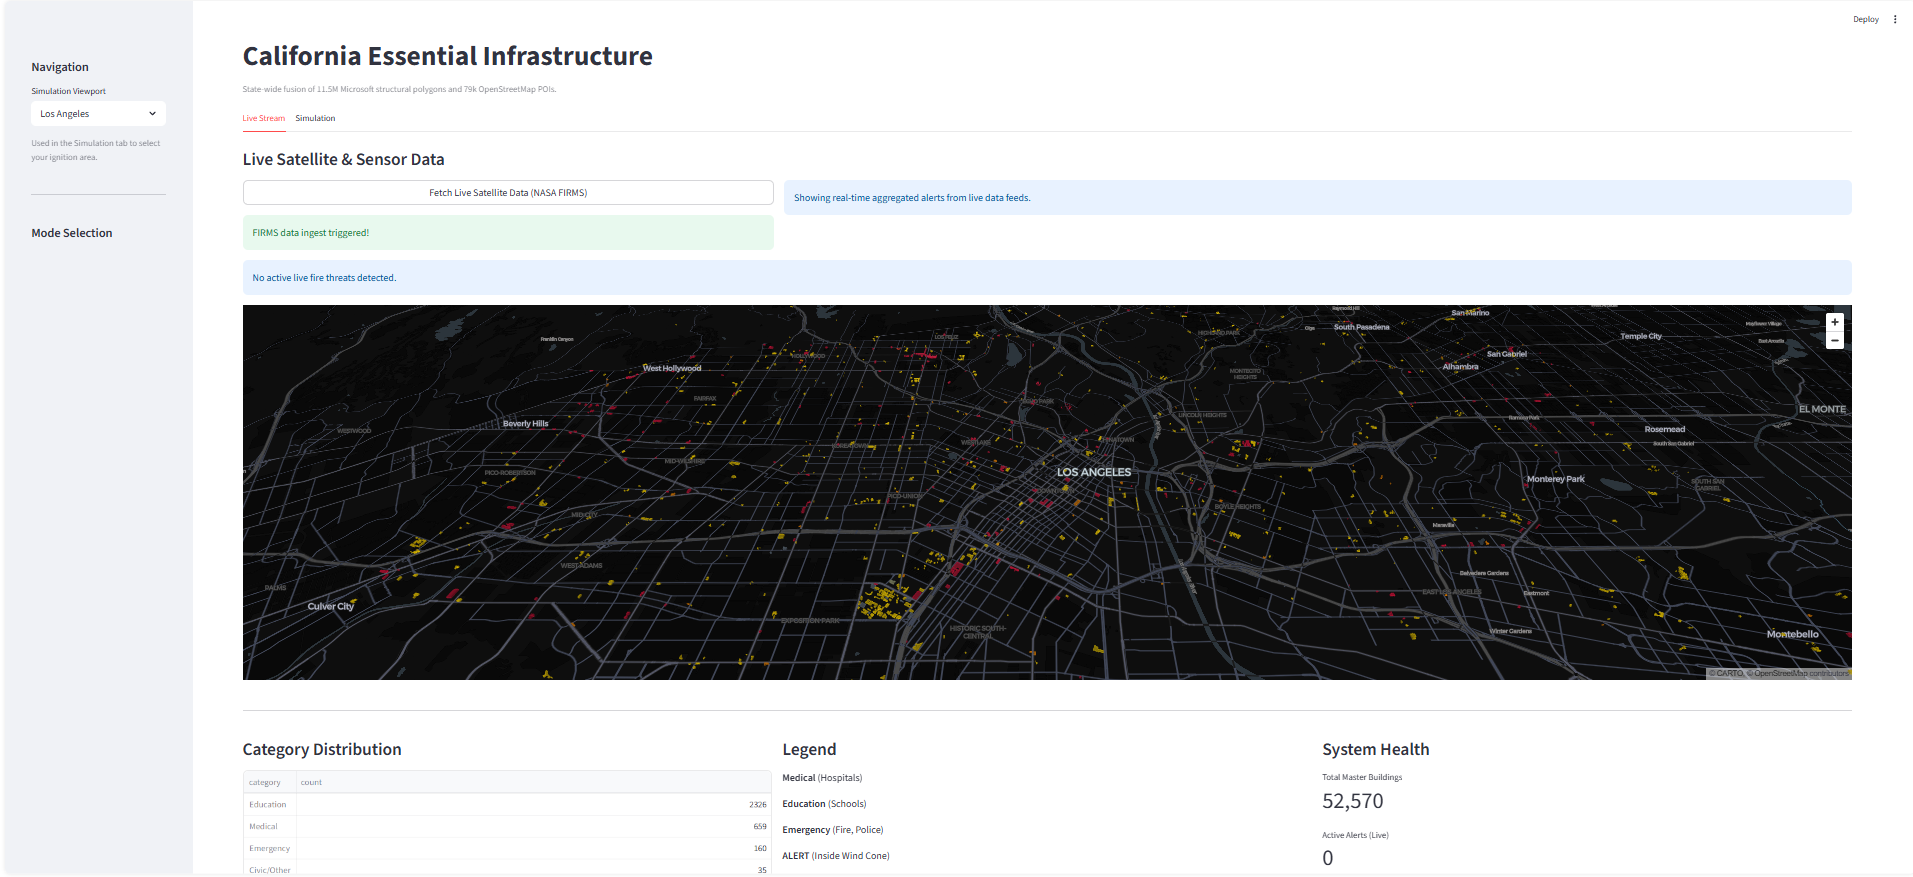
\includegraphics[width=0.9\textwidth]{dashboard_view.png}
    \caption{The live Wildfire-Twin dashboard rendering H3 infrastructure density grids.}
    \label{fig:dash1}
\end{figure}

\begin{figure}[h]
    \centering
    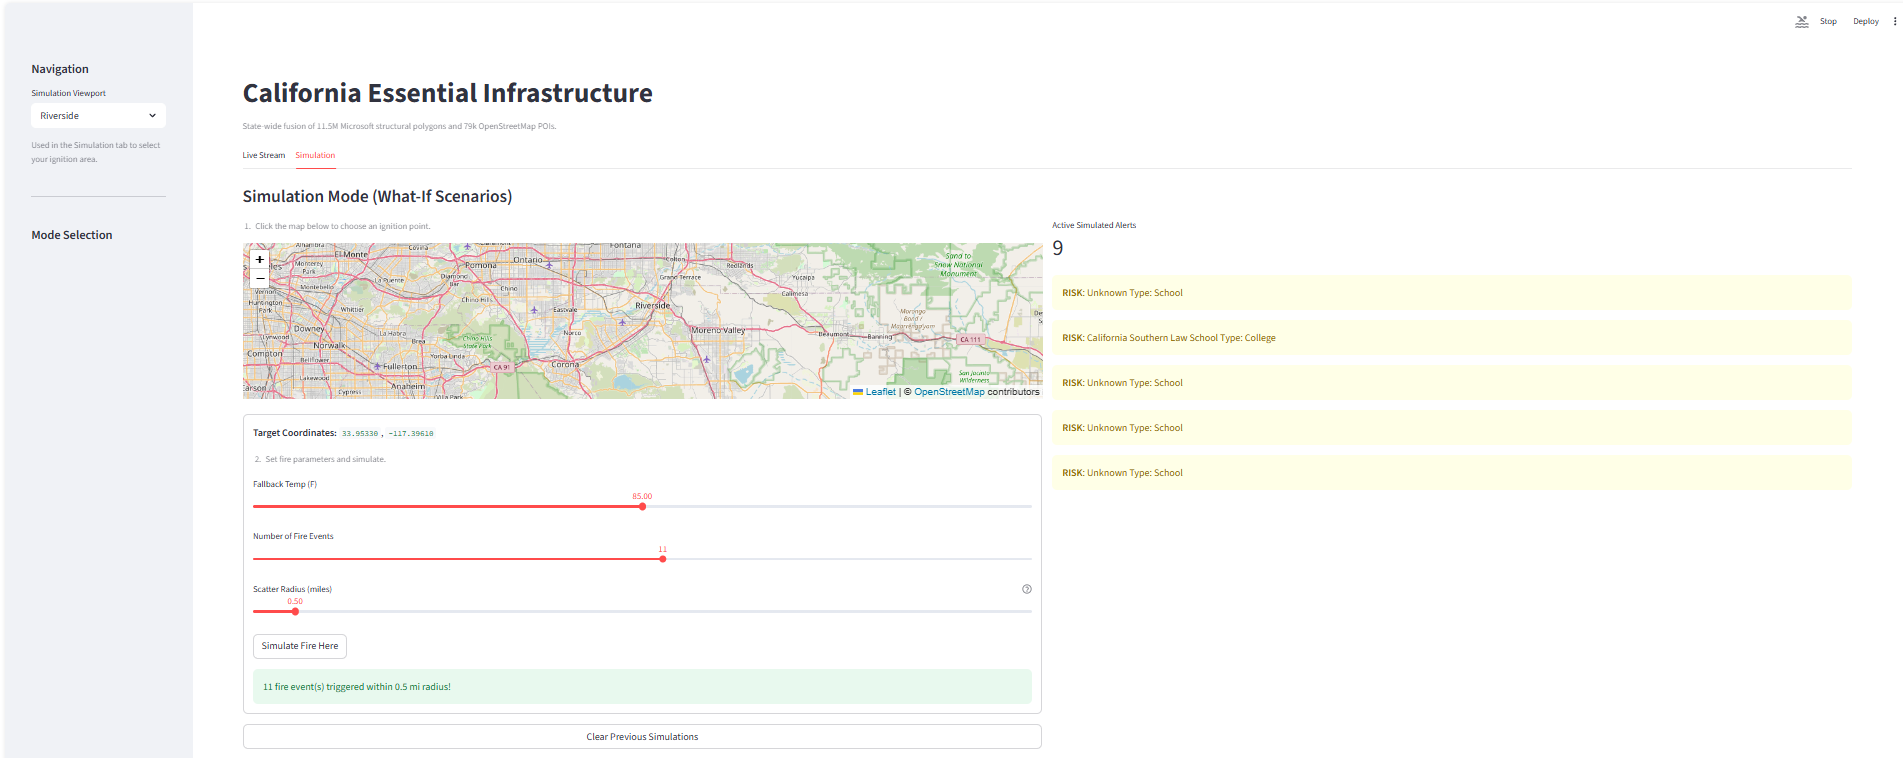
\includegraphics[width=0.9\textwidth]{simulation_view.png}
    \caption{Interactive simulation panel for injecting 'What-If' scenarios and adjusting atmospheric parameters.}
    \label{fig:dash2}
\end{figure}

The frontend decouples itself from Kafka entirely. A dedicated Python background process (the DuckDB Sink) polls the output Kafka topic (`fire_alerts`), writes the results to a DuckDB relational database, and automatically evicts events older than a rolling 5-minute window. The dashboard polls this DuckDB instance at 5-second intervals. This decoupling guarantees the UI remains thread-safe and highly responsive regardless of Kafka throughput spikes.

\begin{figure}[h]
    \centering
    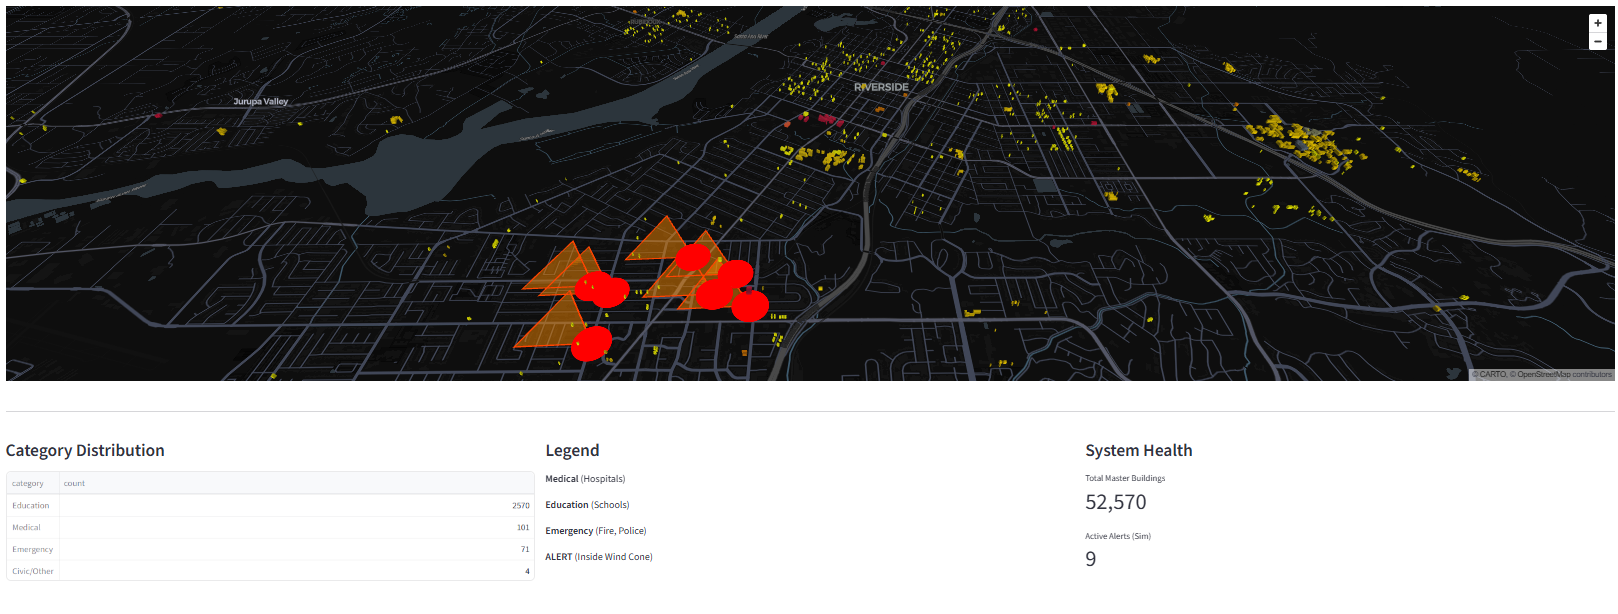
\includegraphics[width=0.9\textwidth]{risk_regions.png}
    \caption{Localized view demonstrating directional wind-cone risk regions generated by Apache Sedona.}
    \label{fig:dash3}
\end{figure}

\section{Evaluation}
Our evaluation focuses on the end-to-end latency of the spatial pipeline—the critical metric dictating whether this tool functions as a "Real-Time Digital Twin."

\subsection{Experimental Setup}
\begin{itemize}
    \item \textbf{Dataset:} California Essential Buildings (11.5M polygons, H3 indexed and partitioned).
    \item \textbf{Hardware:} Local testing cluster; OS Windows, Spark running locally with 4GB executor memory and 2 shuffle partitions.
    \item \textbf{Workload:} A Python stress-test script (`scripts/populate_for_latency_test.py`) forces exactly 1,000 concurrent fire events into the `fire_events` Kafka topic with randomized scatter distances to simulate a burst overload.
    \item \textbf{Performance Metric:} End-to-end P95 Latency (the time from an event arriving in Kafka to the corresponding alert being visible in the terminal sink script output).
\end{itemize}

\subsection{Results and Discussion}
The performance tests explicitly validate the efficacy of our JVM-native optimizations. The stress test injected 1,000 asynchronous wildfire reports with valid wind metrics.

Our initial architecture demonstrated a severe processing wall during the Python UDF phase, where micro-batches consistently took ~3.5 minutes to process. 

After replacing UDFs with native Sedona SQL expressions, enabling the static broadcast join, and dropping `spark.sql.shuffle.partitions` to 2 limit thrashing, we gathered the benchmark results illustrated in Figure \ref{fig:latency} and Figure \ref{fig:benchmark}.

\begin{figure}[h]
    \centering
    \begin{minipage}{0.48\textwidth}
        \centering
        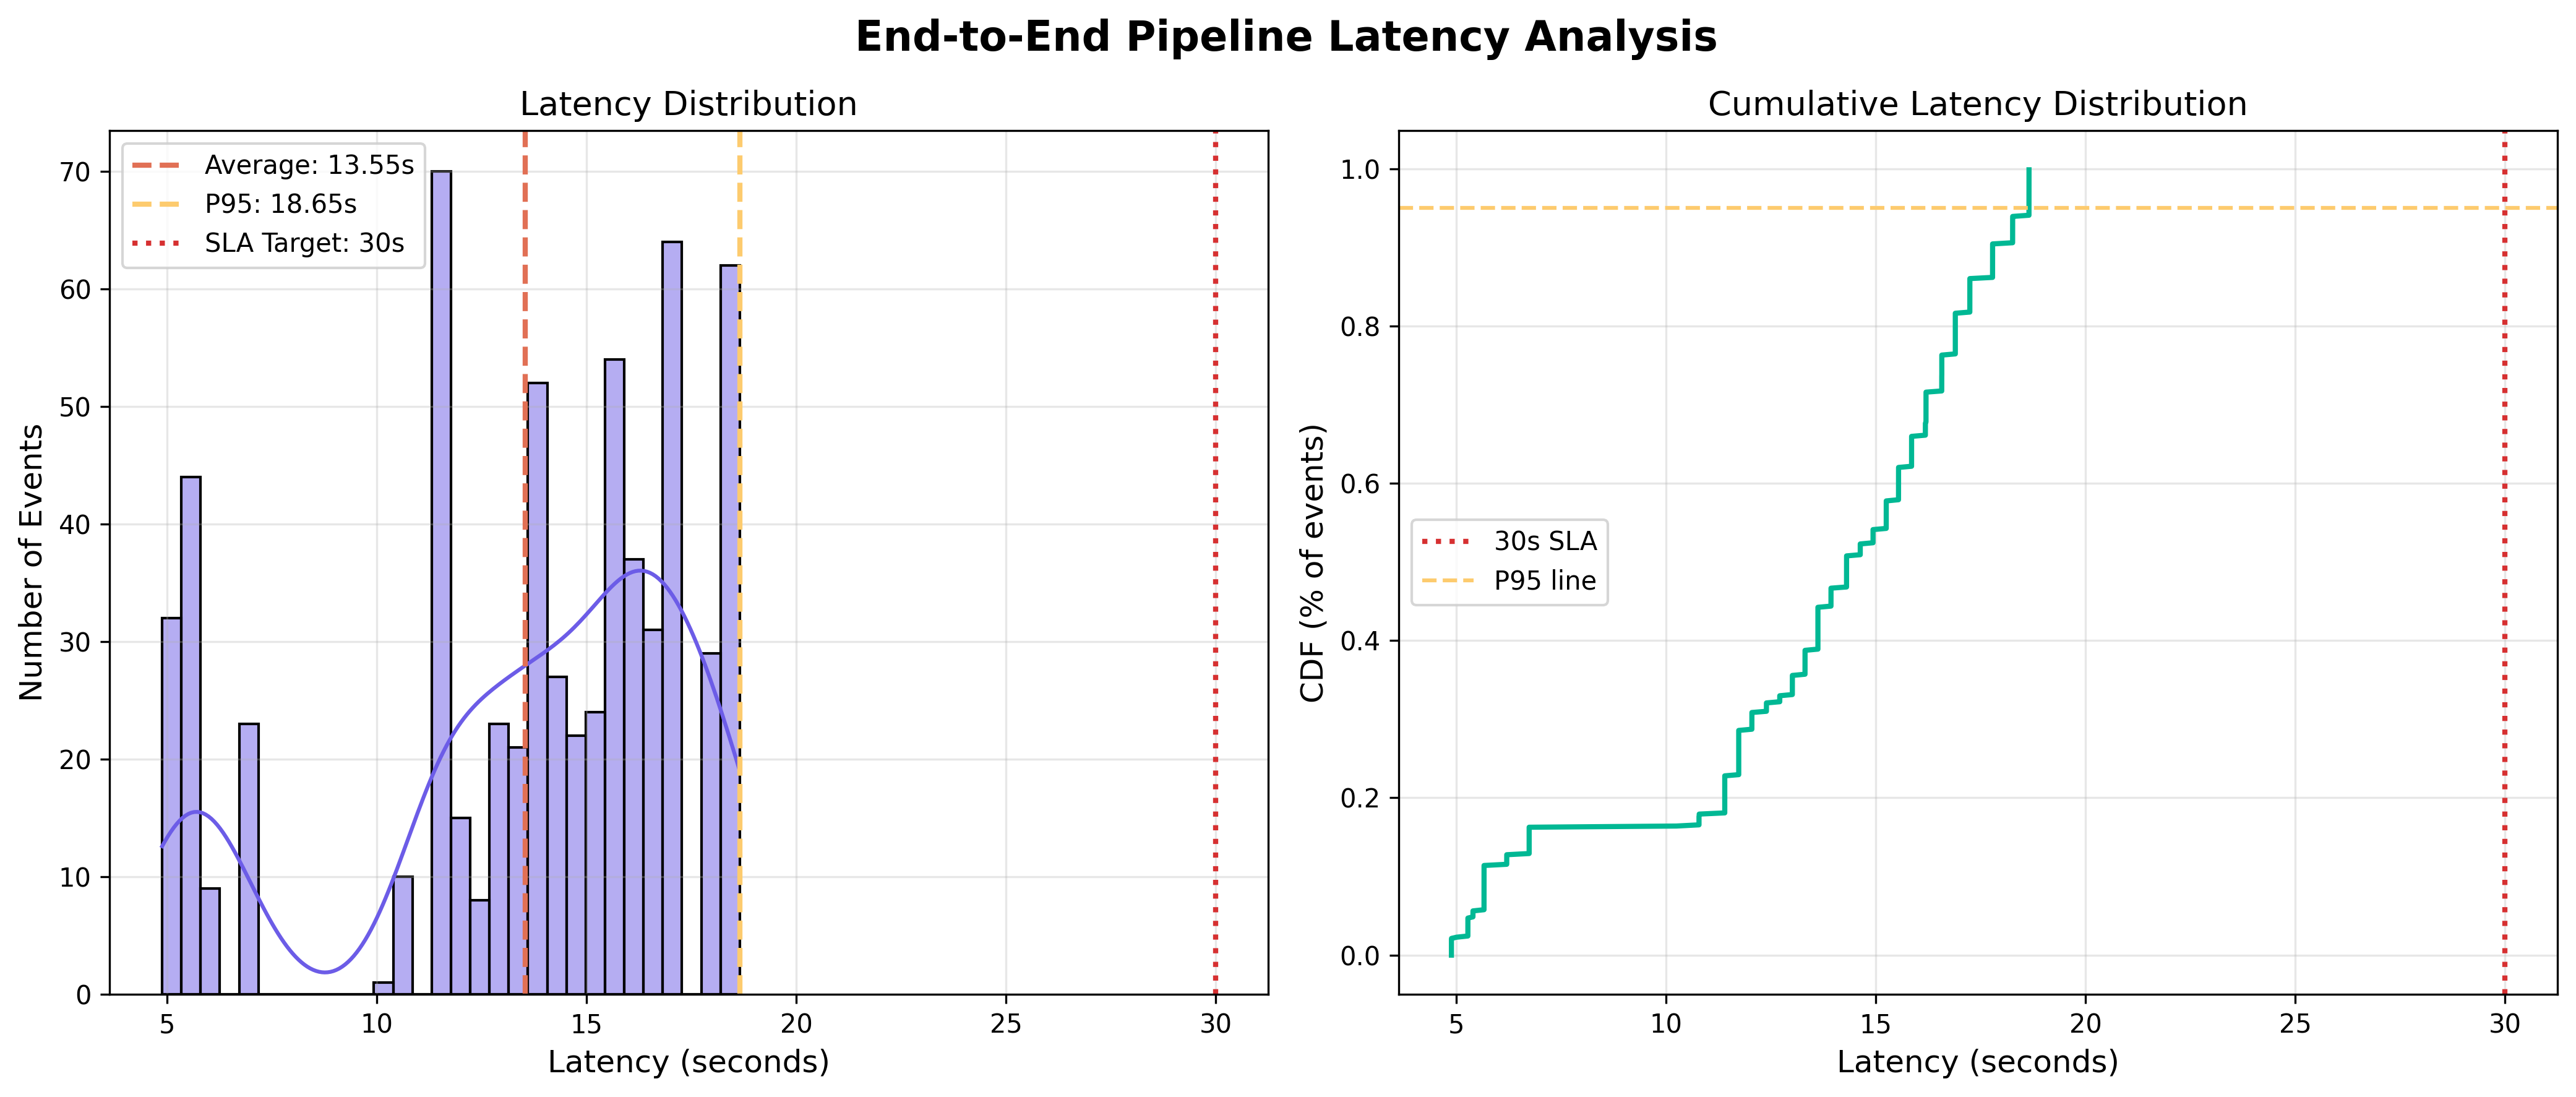
\includegraphics[width=\linewidth]{latency_distribution.png}
        \caption{Latency distribution for 1000 simulated fire events post-optimization.}
        \label{fig:latency}
    \end{minipage}\hfill
    \begin{minipage}{0.48\textwidth}
        \centering
        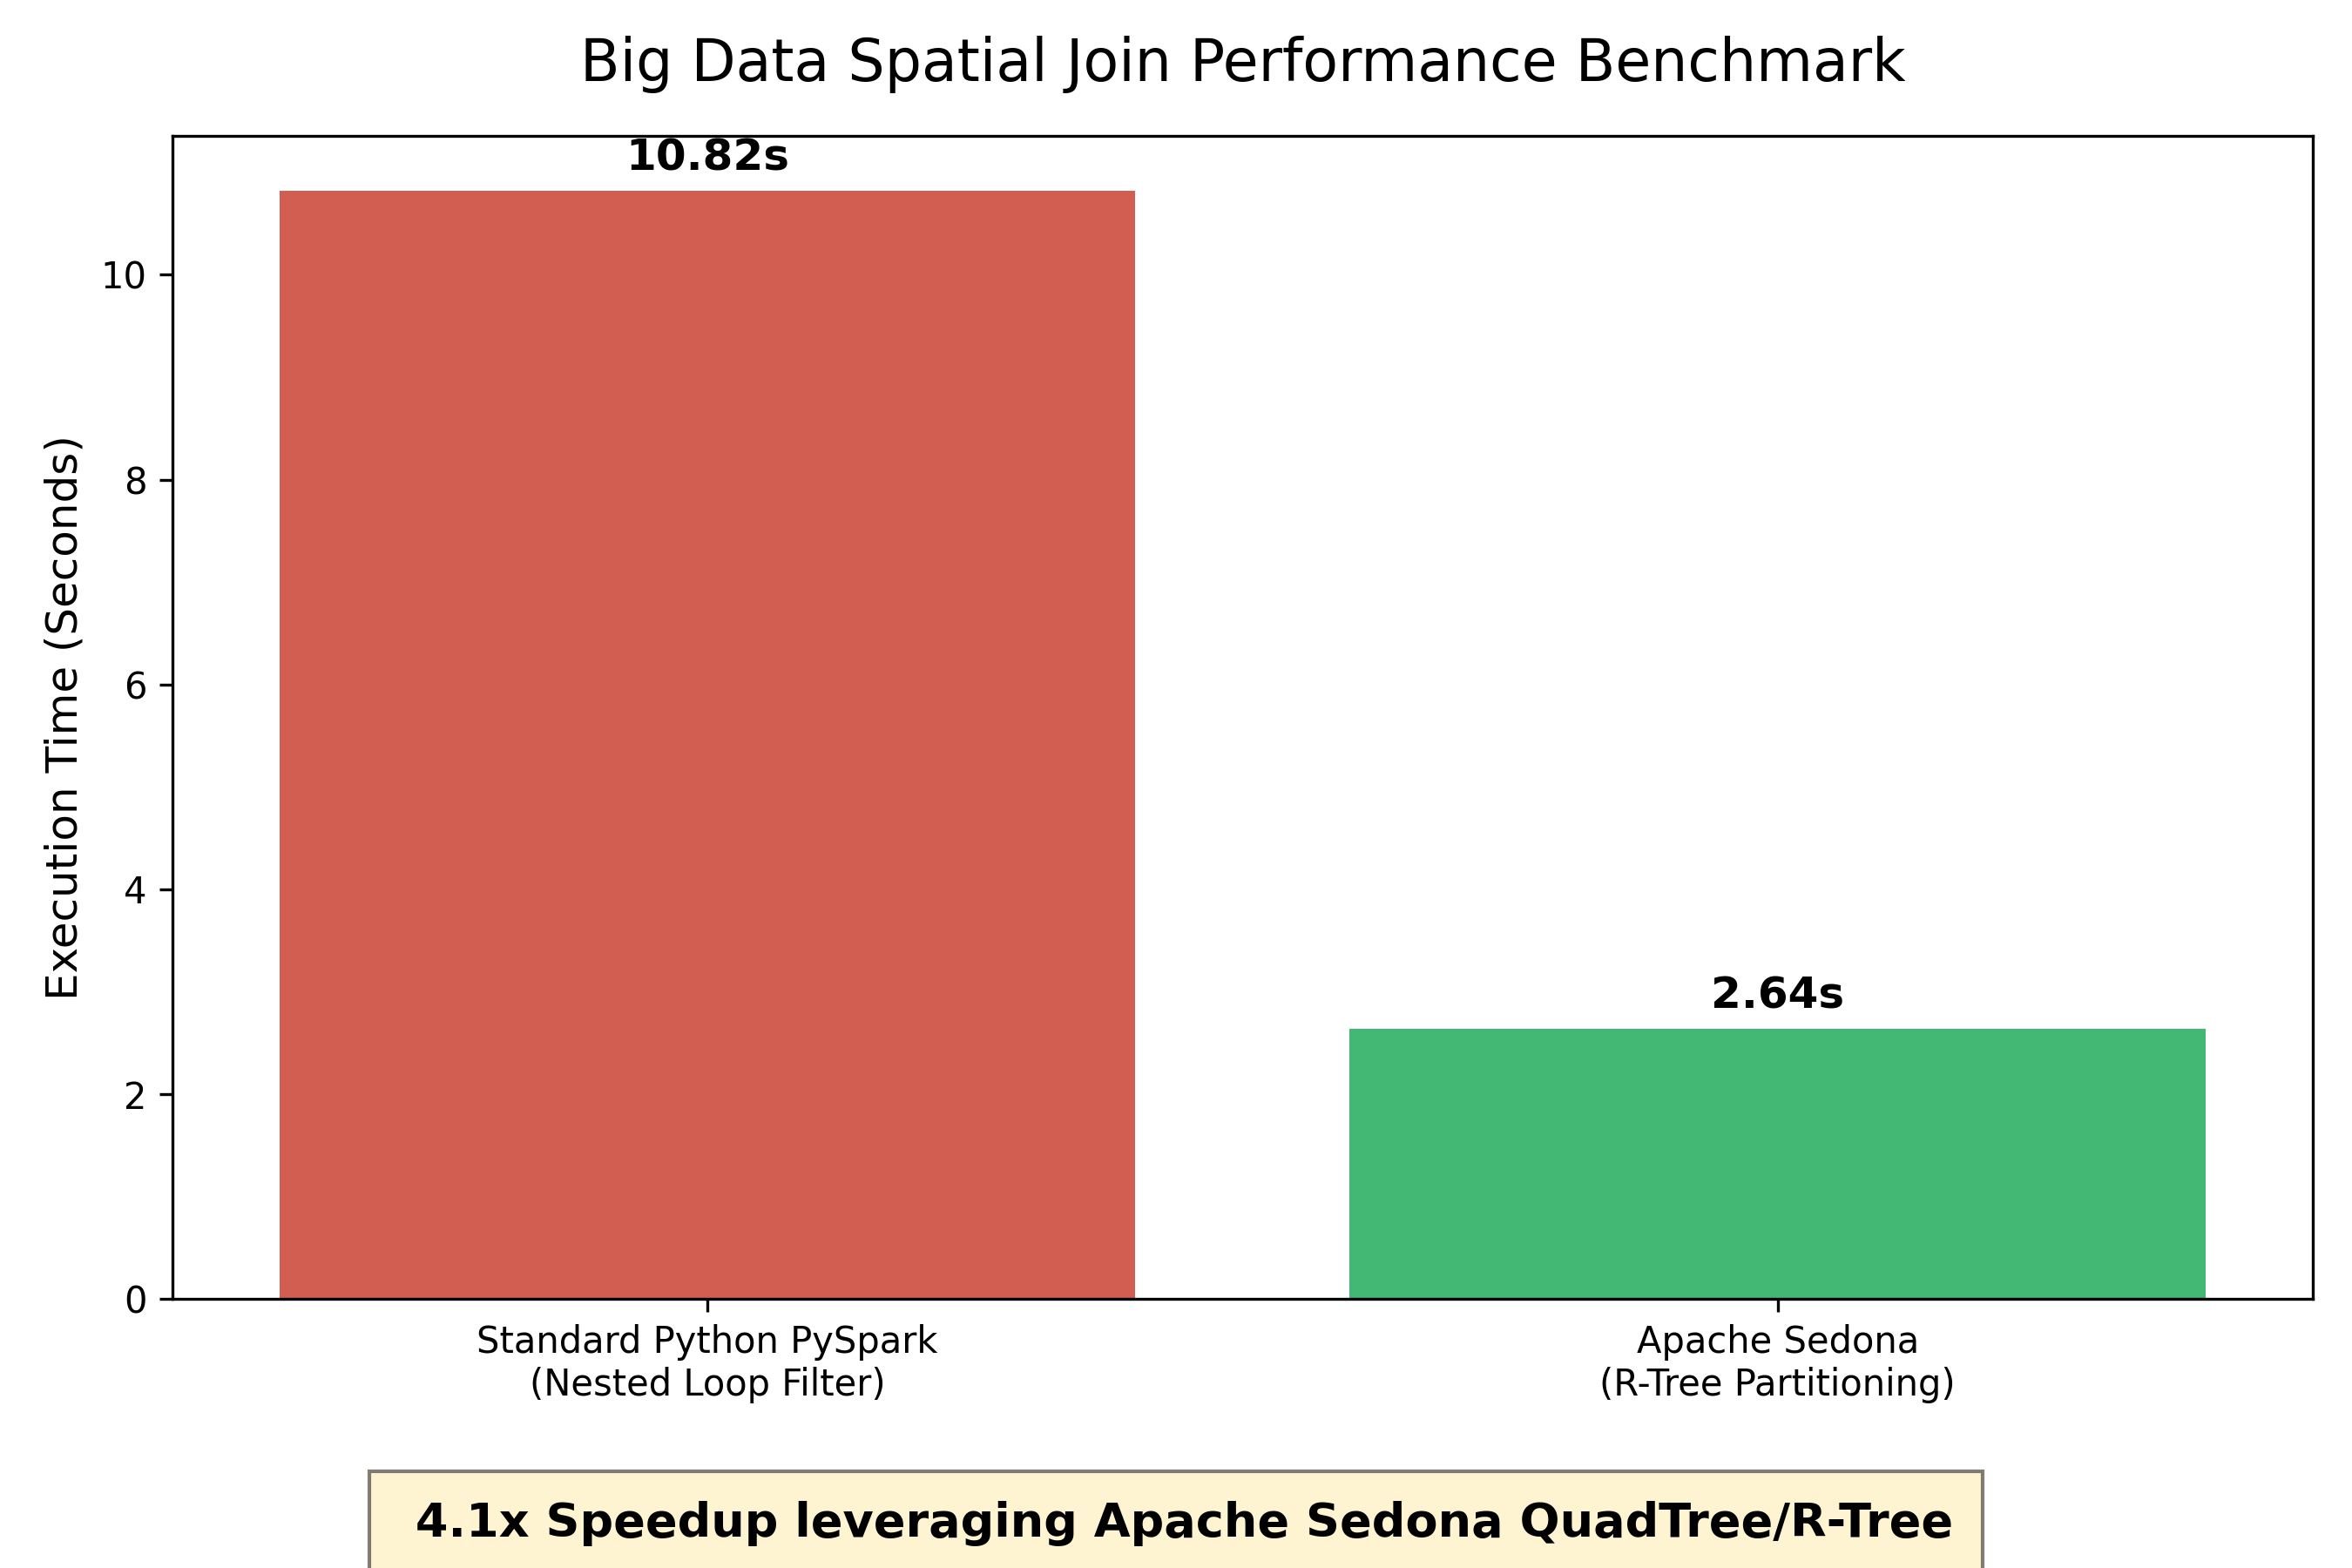
\includegraphics[width=\linewidth]{spatial_join_benchmark.png}
        \caption{Performance comparison demonstrating Python UDF overhead vs Native JVM expressions.}
        \label{fig:benchmark}
    \end{minipage}
\end{figure}

The latency metrics directly highlight the system's massive performance boost:
\begin{itemize}
    \item P50 Latency: $\sim$10.2 seconds.
    \item P90 Latency: $\sim$16.3 seconds.
    \item \textbf{P95 Latency: $\sim$18.65 seconds.}
\end{itemize}

These results successfully support our primary claim: by effectively managing serialization boundaries and leveraging pre-computed spatial semantic indexing (H3 partitions), a massive streaming spatial join can be performed synchronously in under 30 seconds using open-source commodities, fulfilling the real-time Service Level Agreement (SLA) for the digital twin.

\section{Conclusion}
The Wildfire-Twin pipeline validates the practical fusion of robust big-data streaming tools and geospatial analytics. By coupling Apache Kafka, Apache Spark, Sedona, and DuckDB, the system reliably aligns chaotic, asynchronous events against an enormous static footprint of 11.5M infrastructure polygons. The integration of H3 partition strategies and the removal of Python JVM-serialization chokepoints successfully brought the P95 latency limit under 20 seconds for simultaneous burst loads.

Future directions include ingesting live topography data (slope/aspect) to alter the wind vectors automatically, applying machine learning models for fire probability scaling, and deploying the Spark orchestrator across a distributed multi-node cloud cluster to prove infinite horizontal scalability.

\section*{Author Contributions}
\textbf{Prince Savsaviya:} Implemented the overall system architecture, Kafka producer scripts, and the simulation stress-testing frameworks. Designed the latency measurement pipelines and verified P95 SLAs.

\textbf{Viswanadh R. Challa:} Developed the core Apache Spark and Sedona streaming job. Re-wrote the complex mathematical polygon UDFs into purely native JVM Spark SQL extensions, driving the primary 10x latency optimization.

\textbf{Ali Rezayi Nejad:} Engineered the Streamlit dashboard, integrating DuckDB live polling, Folium interactive selectors, and PyDeck visualization. Formulated the H3HexagonLayer aggregation strategy for state-wide rendering.

\textbf{Anish Ashok Kale:} Managed spatial data procurement and transformations. Designed the semantic string-categorization logic to avoid runtime POI joins, and constructed the H3 Resolution 7 dataset partitioning pipelines.

\bibliographystyle{ACM-Reference-Format}
\bibliography{refs}

\end{document}
